%\epigraph{Yesterday's rose stands only in name, we hold only empty names.}{--- \textup{Umberto Eco}, \textit{The Name of Rose}}
This Chapter introduces the properties of neutrinos and their interactions, focusing on the weak interactions, neutrino mass and flavor transformations. 

Since the first discovery of the neutrinos in the 1950s, different types of neutrino experiments have measured and studied neutrinos produced from different sources, which are mainly: the core of the Sun, the Earth's mantle and crust, the atmosphere, fission reactors, accelerator beams, and astrophysical objects, such as supernovae in space. These sources produce solar neutrinos, geoneutrinos, atmospheric neutrinos, reactor antineutrinos, accelerator neutrinos and supernova/astrophysical neutrinos respectively. Among them, the experiments measuring solar neutrinos have unraveled the phenomenon of neutrino flavor transformations in the matter. The solar neutrino experiments relevant to the analysis presented in Chapter 6 are introduced. The rest of the Chapter introduces the major physics target for SNO+: the neutrinoless double beta decay, and the relevant experiments.

\section{Neutrinos}

A neutrino is a spin-1/2 fermion with a neutral electric charge and only interacts via weak interaction and gravity. Its basic properties and interactions are described by the Standard Model (SM), a theory describing the properties of all elementary particles currently observed and their interactions based on the three fundamental forces: the strong, weak, and electromagnetic forces. Notably, gravity as one of the fundamental forces is not included in the SM, and it still waits for a new theory. 

The SM has successfully explained and predicted phenomena in particle physics since the latter half of the 20th century. An important triumph achieved by the SM is the discovery of the predicted Higgs bosons in 2012. However, there are still open issues in the SM. Besides the notable gravity issue, some of the unsolved questions are relating to the mystery properties and behaviors of neutrinos: What are the masses of neutrinos? How do neutrinos obtain their masses? Why are their masses so small compared to the other elementary particles? Are neutrinos their own antiparticles? And there might be more questions about neutrinos coming out. If any of these questions is answered, a door will be opened to the new physics theories beyond the SM.

Since neutrinos weakly interact with other particles and fields, they can penetrate through massive matter or travel a long way through space without being interrupted. Neutrinos produced in the core of the Sun, in Supernovae, or in the galactic core of the Milky Way can carry original information of these astrophysics objects and easily bring these information to the detectors on the Earth. This property enables neutrinos as a probe to study the status of astrophysics objects.

The interesting facts mentioned above put the researches of neutrinos under the spotlight. 

The existence of neutrinos was first put forward by Wolfgang Pauli in the 1930s to solve the observed contradicts in $\beta$-decay process. In 1914, James Chadwick found that the electrons emitted in $\beta$-decay (called the ``$\beta$-electrons'') have a continuous energy spectrum\cite{leite1996weak}. However, since nuclei have discrete energy levels, the energy spectrum of $\beta$-electrons should be discrete and equal to the difference between the final and initial states of nuclei. This indicates that the energy and momentum are not conserved if only nuclei and $\beta$-electrons present in the $\beta$-decay products. Pauli then introduced a charge-neutral, spin-1/2, and nearly massless particle to the $\beta$-decay products. This particle was later called ``neutrino'' (the small neutral one) by Enrico Fermi. The neutrinos take away a part of energies and then cause the broad energy spectrum of $\beta$-electrons, thus the problem was solved.

In 1934, Fermi developed the four-fermion vertex interaction theory to describe the weak interactions relating to neutrinos. Soon after that, Bethe and Peierls suggested direct neutrino detection can be made via a neutrino-induced interaction, called the inverse beta decay (IBD): $\bar{\nu}_e+p\to e^+ + n$. Their calculation showed that the IBD cross-section was in the order of $(10^{-44})$ cm$^2$, which was difficult for detection\cite{bethe1934neutrino}. Though the task to detect neutrinos was difficult, in 1956, Fred Reines and Clyde Cowan made the first discovery of the antineutrinos from nuclear reactors. They measured the cross-section as $6.3\times10^{-44}$ cm$^2$, which was consistent with Bethe's calculation\cite{reines1960detection}.

In 1962, Lederman, Schwartz, and Steinberger demonstrated that more than one type of neutrino exists by detecting the interactions of the muon neutrino ($\nu_\mu$)\cite{danby1962observation}. The tauon neutrino ($\nu_\tau$) was proposed after the discovery of the $\tau$ lepton and was observed in 2000 by the DONUT collaboration\cite{kodama2001observation}. The decay width of the $Z^0$ boson measured by the ALEPH collaboration implied that based on the SM, the number of light neutrino species is three\cite{decamp1989determination}.

Currently, we know that neutrinos have three leptonic flavors, and they only participate in the weak and gravitational interactions, while the latter can be neglected in the particle-scale. In the weak interactions, a neutrino $\nu_\alpha$ is generated with a definite leptonic flavor, accompanied by one of the three charged leptons: electron ($e$), muon ($\mu$) or tauon ($\tau$). It is identified as an electron neutrino ($\nu_e$), a muon neutrino ($\nu_\mu$), or a tauon neutrino ($\nu_\tau$).

The weak interactions are described in the SM by fermions exchanging $W^{\pm}$ and $Z^0$ bosons known as weak force carriers. 

% The charged-current (CC) interaction is mediated by the charged vector bosons $W^\pm$, while the neutral-current (NC) is mediated by the neutral vector boson $Z^0$.

In the SM, only the left-handed neutrino and right-handed antineutrino can take part in the weak interaction.



lepton number conservation

Neutrino interactions mainly include the neutrino-electron scatterings, hadron decays and neutrino-nucleon scatterings\cite{giunti2007fundamentals}. The next section mainly focuses on the low-energy ($\mathcal{O}$(MeV)) neutrino-electron ($\nu+e^-$) elastic scattering, which plays an important role in the detection of solar neutrinos.

\section{Neutrino-Electron Elastic Scattering}\label{sect:nuInteraction}
The $\nu+e^-$ elastic scattering (ES): $\nu_x + e^{-}\to\nu_x+e^-$ (also for $\bar{\nu}_x$) is a pure leptonic process and can be precisely described by the electroweak theory in the SM. The amplitude for this process is contributed by both neutral current (NC) and charged current (CC) interactions. Fig.~\ref{fig:feynman-es} shows the tree-level Feynman diagrams (without radiative corrections).

The $\nu+e^-$ ES is sensitive to all neutrino flavors, but the $\nu_e$ can undergo CC (exchanging W boson) (as shown in Fig.~\ref{fig:feynman-es}) and NC (exchanging $Z^0$ boson) interactions, whereas $\nu_\mu$ and $\nu_\tau$ interact only through the
NC. 

for the neutrinos with $\mathcal{O}$(10 MeV) energy, especially the solar neutrinos (will be discussed in Sect.~\ref{sect:solarNu}), 


\begin{figure}[htbp]
	\centering
	\begin{minipage}[t]{0.45\textwidth}{(a)}
		\centering
		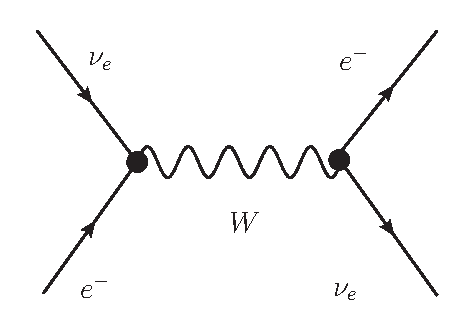
\includegraphics[width=4.5cm]{charged-1.eps}
	\end{minipage}
	\begin{minipage}[t]{0.3\textwidth}{(b)}
		\centering
		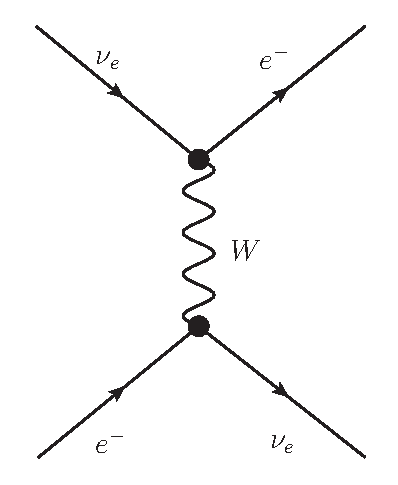
\includegraphics[height=4cm]{charged.eps}
	\end{minipage}
	\begin{minipage}[t]{0.4\textwidth}{(c)}
		\centering
		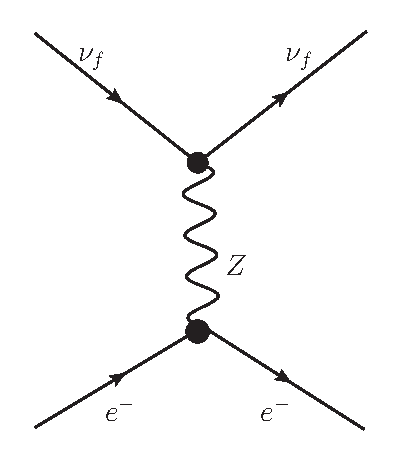
\includegraphics[height=4cm]{neutral.eps}
	\end{minipage}
	\caption[Feynman diagrams for the elastic scattering interaction in different channels at tree level.]{Feynman diagrams for the elastic scattering interaction in different channels at tree level. (a) and (b): CC for s and t channels, respectively; (c): NC.}
	\label{fig:feynman-es}
\end{figure}

In a particle detector, the electron is usually from the atom of detection medium. 
conservation of momentum.
In the laboratory frame, the kinetic energy of a recoil electron from the $\nu+e^-$ ES process is\cite{giunti2007fundamentals}:
\begin{equation}
T_e = \frac{2m_eE_\nu^2\cos^2\theta}{(m_e+E_\nu)^2-E_\nu^2\cos^2\theta},
\end{equation}
where the scattering angle $\theta$ is between the momentum directions of the incoming neutrino and the scattered or recoil electron, as shown in Fig.~\ref{fig:ESdiagram}.

\begin{figure}[htbp]
	\centering	
	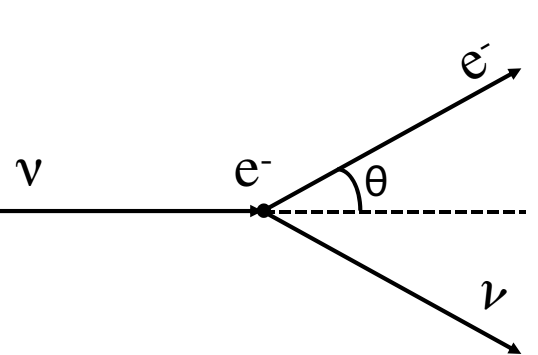
\includegraphics[width=6cm]{ElasticScatteringCartoon.png}
	\caption{A diagram of the $\nu + e^-$ elastic scattering in the lab frame, modified from Ref.~\cite{giunti2007fundamentals}.	\label{fig:ESdiagram}}
\end{figure}

The direction of the scattered electron is strongly correlated with the direction of the incident neutrino. For solar neutrinos, the scattering angle is denoted as ``solar angle'' ($\theta_{sun}$) in this thesis. It is one of the crucial parameters for measuring solar neutrinos, which will be discussed in Chapter 6 for analyzing solar neutrinos in the SNO+ water phase.

\begin{equation}\label{eq:costhetaSun}
\cos\theta_{sun}=\sqrt{\frac{T_e(m_e+E_\nu)^2}{2m_eE_\nu^2+T_eE_\nu^2}},
\end{equation}

The differential cross section of the $\nu+e^-$ ES in the lab frame (without radiative corrections) is given by\cite{suzuki2020sun,xing2011neutrinos,giunti2007fundamentals}:
\begin{equation}
\frac{d\sigma}{dT_e}(E_\nu,T_e)=\frac{G_F^2m_e}{2\pi}\left[(c_V+c_A)+(c_V-c_A)^2\left(1-\frac{T_e}{E_\nu}\right)^2-(c_V^2-c_A^2)\frac{m_eT_e}{E_\nu^2}\right],
\end{equation}
where the coupling parameters $c_V=(2\sin^2\theta_W\pm\frac{1}{2})$, $c_A=\pm\frac{1}{2}$, $\sin^2\theta_W=0.23$, and the ``$+$'' sign is for the $\nu_e+e^-$ case while ``$-$'' sign is for the $\nu_{\mu,\tau}+e^-$ case.

The maximum energy of the recoil electron is: $T_{max}=\frac{2E^2_\nu}{2E_\nu+m_e c^2}$, and
the cross-section is $\sigma^{ES}(\nu_e e^-)=9.52\times 10^{-44}(E_\nu/10~\mathrm{MeV)~cm^2}$
the expected solar neutrino rate is 
$R=A\int_{T_{thresh}}^{T_{max}}\frac{d\sigma}{dE}\frac{dN}{dE_\nu}dE_\nu$.

The shape of the recoil electron energy spectrum and the directionality are utilized by the experiments to tag solar neutrinos in real-time\cite{suzuki2020sun}. These experiments will be introduced in Sect.~\ref{sect:solarNu}.

For the solar neutrino case, $E_\nu\gg m_e$, the total cross section of $\nu_e+e^-$ ES and $\nu_x+e^-$ ES ($x=\mu$ or $\tau$) can safely approximate to\cite{xing2011neutrinos}:
\begin{equation}
\begin{aligned}
\sigma^{ES}(\nu_e+e^-) = \frac{2G_F^2}{\pi}m_e E_\nu \left[(1+c_L)^2+\frac{1}{3}(c_R)^2\right],\\
\sigma^{ES}(\nu_x+e^-) = \frac{2G_F^2}{\pi}m_e E_\nu \left[(c_L)^2+\frac{1}{3}(c_R)^2\right].
\end{aligned}
\end{equation}
where $x=\mu$ or $\tau$, $c_L=\frac{(c_V+c_A)}{2}$ and $c_R = \frac{(c_V-c_A)}{2}$.

Then the ratio of $\sigma^{ES}(\nu_{\mu,\tau}+e^-)$ to $\sigma^{ES}(\nu_e+e^-)$ is\cite{xing2011neutrinos}:
\begin{equation}
\frac{\sigma^{ES}(\nu_{x} e^-)}{\sigma^{ES}(\nu_e e^-)} = \frac{3(c_L)^2+({c_R})^2}{3(1+c_L)^2+(c_R)^2} \approx 0.155,
\end{equation}

Or, the cross section of the CC ES is about 6.5 times larger than the NC ES. %This indicates that for the experiments measuring the $\nu$ via the $\nu e^-$ ES channel, for the same exposure (detector running time$\time$ active target mass), the number of the measured $\nu_e$ is about 6.5 times the number of $\nu_\mu$ or $\nu_\tau$.  

\section{Neutrino Flavor Transformation}
Neutrino flavor transformation is a quantum mechanical interference phenomenon\cite{akhmedov2019quantum}. It was first discovered in 1998, based on the analysis of atmospheric neutrino fluxes measured by the Super-Kamiokande (Super-K) experiment to solve the ``atmospheric neutrino anomaly''\cite{fukuda1998evidence}. It is the first direct evidence showing that neutrinos have finite masses and the SM is incomplete.

\subsection{Vacuum Oscillation}\label{sect:VacuumOsci}
For neutrino flavor oscillation experiments, neutrinos are detected in certain flavor eigenstates via weak interaction. A neutrino flavor state vector can be taken as a linear superposition of the mass eigenstates. For three-flavor neutrino mixing, we have\cite{pdg2020}:
\begin{equation}\label{eq:mixingmatrix}
|\nu_f\rangle = \sum_{i=1}^3U^*_{fi}|\nu_i\rangle, 
\end{equation}
where $f=e,\mu,\tau$ and $k=1,2,3$. The unitary PMNS matrix, $U_{PMNS}$, can be parameterized as\footnote{Here we ignore the Majorana CP violation phases, which are cancelled out when tackling with the flavor transformation probability. They will be introduced in Sect.~\ref{sect:doublebeta}.}: 
\begin{equation}\label{eq:uPMNS}
U_{PMNS} =
\begin{pmatrix}
1 &0 &0\\
0 &c_{23} &s_{23}\\
0 &-s_{23} &c_{23}\\ 
\end{pmatrix}
\begin{pmatrix}
c_{13} &0 &e^{-i\delta_{CP}}s_{13}\\
0 &1 &0\\
e^{-i\delta_{CP}}s_{13} &0 &c_{13}\\ 
\end{pmatrix}
\begin{pmatrix}
c_{12} &s_{12} &0\\
-s_{12} &c_{12} &0\\
0 &0 &1\\ 
\end{pmatrix},
\end{equation}
where $c_{ij}\equiv \cos\theta_{ij}$ and $s_{ij}\equiv \sin\theta_{ij}~(i,j = 1,2,3)$ are shorthands.
In the PMNS matrix, there are four parameters: the three mixing angles $\theta_{12}$, $\theta_{13}$, $\theta_{23}$ and the charge-parity (CP) violation parameter of lepton sector, $\delta_{CP}$. The unknown value of $\delta_{CP}$ is related to leptogenesis, the hypothetical physical process that produced an asymmetry between leptons and anti-leptons in the very early universe\cite{wiki_cp}. 

Now discuss the vacuum flavor oscillation: in the lab frame, assume a neutrino is generated at time $t_0=0$ from a source with a certain flavor state $|\nu_\alpha\rangle$. It then propagates in vacuum with a speed close to the speed of light (ultra-relativistic) for a distance $L$ and is finally detected at time $t$ in a detector. The flavor eigenstate evolves in space-time is $|\nu_\alpha \rangle = \sum_i U^*_{\alpha i}|\nu_i,p_i\rangle$, where $p_i$ is the 4-momentum of $\nu_i$. The momentum is assumed to be along the direction from the source to the detector and only in one dimension. Via the Schr\"{o}dinger equation, the amplitude for the flavor eigenstate $|\nu_\beta\rangle$ in the detector at $(L,t)$ is (use the natural units: $\hbar=c=1$) \cite{aitchison2012gauge}:
\begin{equation}
\mathcal{A}(\nu_\alpha\to\nu_\beta;L,E)=\sum_{i}U^*_{\alpha i}e^{-iE_i t+ip_iL}\langle\nu_\beta|\nu_i,p_i\rangle=\sum_{i}U^*_{\alpha i}U_{\beta i}e^{-iE_it+ip_iL},
\end{equation}

Then the probability of $\nu_\alpha$ at time $t_0=0$ transforms into a $\nu_\beta$ at time $t$ is:
\begin{equation}\label{oscillationEq1}
 \begin{split}
&P(\nu_\alpha\to\nu_\beta;L,E)=|\langle\mathcal{A}(\nu_\alpha\to\nu_\beta;L,E)|\mathcal{A}(\nu_\alpha\to\nu_\beta;L,E)\rangle|^2=\\
&(U^*_{\alpha 1}U_{\beta 1}e^{-iE_1t+ip_1L}+U^*_{\alpha 2}U_{\beta 2}e^{-iE_2t+ip_2L}+...)(U_{\alpha 1}U^*_{\beta 1}e^{+iE_1t-ip_1L}+U_{\alpha 2}U^*_{\beta 2}e^{+iE_2t-ip_2L}+...)=\\
&\sum_i |U_{\alpha i}|^2|U_{\beta i}|^2 + \sum_{i>j}(U^*_{\alpha i}U_{\beta i}U_{\alpha j}U^*_{\beta j})\exp\{-i(E_i-E_j)t+i(p_i-p_j)L\}+(i\leftrightarrow j),
\end{split}
\end{equation}
where $(i\leftrightarrow j)$ stands for the second term exchanging the $i,j$ indices.

For the second term in Eqn.~\ref{oscillationEq1}, in the ultra-relativistic case, $p_i\simeq p_j\equiv p\simeq E\gg m$, where $E$ is the average energy. Then $E_i=\sqrt{p^2_i+m^2_i}\simeq p+\frac{m_i^2}{2E}$ and thus $E_i-E_j\simeq \frac{m^2_i-m^2_j}{2E}\equiv \frac{\Delta m^2_{ij}}{2E}$\cite{pdg2020,aitchison2012gauge}. Here $\Delta m^2_{ij}$ is a set of parameters called mass square difference, popping out in the flavor transition probability. Along with $L\simeq ct=t~(c\equiv 1)$, we have $\exp\{-i(E_i-E_j)t+i(p_i-p_j)L\}\simeq \exp\{-i\frac{\Delta m^2_{ij}}{2E}\}$. In addition, $U^*_{\alpha i}U_{\beta i}U_{\alpha j}U^*_{\beta j}=|U^*_{\alpha i}U_{\beta i}U_{\alpha j}U^*_{\beta j}|\exp\{i\phi_{\alpha\beta;ij}\}$, where $\phi_{\alpha\beta;ij}=\mathrm{Arg}(U^*_{\alpha i}U_{\beta i}U_{\alpha j}U^*_{\beta j})$ and $\phi_{\alpha\beta;ij}=-\phi_{\alpha\beta;ji}$. Then combine the second term and the $(i\leftrightarrow j)$ term, \ref{oscillationEq1} can be written as\cite{aitchison2012gauge}:
\begin{equation}\label{oscillationEq2}
P_{\nu_\alpha\to\nu_\beta}(L,E)=
\sum_i |U_{\alpha i}|^2|U_{\beta i}|^2 + 2\sum_{i>j}|U^*_{\alpha i}U_{\beta i}U_{\alpha j}U^*_{\beta j}|\cos(\frac{\Delta m^2_{ij}}{2E}L-\phi_{\alpha\beta;ij}).
\end{equation}

Further expand the second term in Eqn.~\ref{oscillationEq2}:
\begin{equation}
 \begin{split}
&|U^*_{\alpha i}U_{\beta i}U_{\alpha j}U^*_{\beta j}|\{\cos(\phi_{\alpha\beta;ij})\cos(\frac{\Delta m^2_{ij}}{2E}L)+\sin(\phi_{\alpha\beta;ij})\sin(\frac{\Delta m^2_{ij}}{2E}L)\}=\\
&\Re(U^*_{\alpha i}U_{\beta i}U_{\alpha j}U^*_{\beta j})(1-2\sin^2\frac{\Delta m^2_{ij}L}{4E})+\Im(U^*_{\alpha i}U_{\beta i}U_{\alpha j}U^*_{\beta j})\sin\frac{\Delta m^2_{ij}L}{2E},
 \end{split}
\end{equation}

since the matrix $U$ is unitary and when $t=0$, 
\begin{equation}
P_{\nu_\alpha\to\nu_\beta}=\delta_{\alpha\beta}=\sum_i |U_{\alpha i}|^2|U_{\beta i}|^2+2\sum_{i>j}\Re(U^*_{\alpha i}U_{\beta i}U_{\alpha j}U^*_{\beta j}),
\end{equation} 

finally it comes out the commonly used vacuum oscillation equation\cite{pdg2020,aitchison2012gauge}:
\begin{equation}\label{common_oscillation}
P_{\nu_\alpha\to\nu_\beta}(L,E)=\delta_{\alpha\beta}-4\sum_{i>j} \Re[U_{\beta i}U^*_{\alpha i}U_{\alpha j}U^*_{\beta j}]\sin^2\frac{\Delta m^2_{ij}L}{4E}+2\sum_{i>j} \Im(U_{\beta i}U^*_{\alpha i}U_{\alpha j}U^*_{\beta j})\sin\frac{\Delta m^2_{ij}L}{2E}.
\end{equation}

Choosing a set of units commonly used by experiments and with dimensional transformation, we have\cite{pdg2020}:
\begin{equation}\label{oscillationCondition}
X_{ij}\equiv \frac{\Delta m^2_{ij}L}{4E}=\frac{1.267\Delta m_{ij}^2[\mathrm{eV}^2]L[m]}{E_\nu[\mathrm{MeV}]}.
\end{equation}

Maximum oscillation occurs when $X_{ij}\sim \pi$, which gives an effective length $L^{osc}(\Delta m_{ij},E_\nu)=4\pi E/|\Delta m_{ij}^2|$.

Currently, the four parameters in the PMNS matrix, as well as the parameters of the $\Delta m_{ij}$, have been measured by neutrino oscillation experiments. These experiments can be classified by the neutrino sources they use. They are the solar, the reactor, the atmospheric, the accelerator, and the astronomical and cosmological neutrino experiments. Table~\ref{nu_exp} lists the energy scale of the neutrino source as well as the example experiments.

\begin{table}[ht]
	\caption{Neutrino experiments for studying flavor transformation.\label{nu_exp} }	
	{\centering
		\begin{tabular*}{135mm}{c@{\extracolsep{\fill}}cccc}
			\toprule 
			type & source & $E_\nu$ & example\\
			\midrule
			solar& the Sun & MeV scale & SNO \\
			reactor& reactor & MeV scale & DayaBay \\
			atmospheric& cosmic-ray& GeV scale & SuperK\\
			accelerator&  $\nu$ beam from accelerator & GeV scale & T2K\\	
			astronomical& astronomical objects & GeV-EeV scale & IceCube\\
			\bottomrule	
		\end{tabular*}
	}
\end{table}

For the $\Delta m^2_{21}$ and $\theta_{12}$, a combined analysis of the measurements from the reactor experiment KamLAND (Kamioka Liquid Scintillator Antineutrino Detector) and the solar neutrino experiment SNO (Sudbury Neutrino Observation) gave $\Delta m^2_{21} = 7.59^{+0.21}_{-0.21}\times 10^{-5}eV^2$ and $\tan^2{\theta}_{21}=0.47^{+0.06}_{-0.05}$\cite{abe2008precision}. Details will be discussed in Sect.\ref{sect:solarNu}.

The accelerator neutrino experiments as well as the atmospheric neutrino experiments have measured $\Delta m^2_{32}$ and $\theta_{23}$. The most recent results from Super-K show that in NH, $\sin^2\theta_{23}=0.588^{+0.031}_{-0.064}$ and $\Delta m^2_{32} = 2.5^{+0.13}_{-0.20}\times 10^{-3} eV^2$\cite{abe2018atmospheric}. 

In 2012, the reactor neutrino experiment Daya Bay reported the discovery of non-zero $\theta_{13}$ with a significance of 5.2$\sigma$. In 2016, Daya Bay reported that $\sin^2 2\theta_{13} = 0.0841\pm0.0027(stat.)\pm0.0019(syst.)$. This high-precision result makes $\sin^2 2\theta_{13}$ the best measured mixing angle\cite{an2017measurement,qian2019physics}.

In addition, there are two squared-mass differences, $\Delta m^2_{21}=m_2^2-m_1^2$ and $\Delta m^2_{32}=|m_3^2-m_2^2|$. The sign of $\Delta m^2_{32}$ is unknown and it indicates a mass hierarchy problem of whether neutrino mass is normal hierarchy (NH, $m_3>m_2>m_1$) or inverted hierarchy (IH, $m_3<m_1<m_2$)\cite{pdg2020}. 

In the case of antineutrino flavor oscillation, we have: $|\bar{\nu}_\alpha\rangle=\sum_i U_{\alpha i}|\bar{\nu}_i,p_i\rangle$, via the same calculation, a similar oscillation probability equation can be found but with the last term in \ref{common_oscillation} being negative\cite{aitchison2012gauge}:
\begin{equation}\label{antiNu_eq1}
P_{\bar{\nu}_\alpha\to\bar{\nu}_\beta}(L,E)=\delta_{\alpha\beta}-4\sum_{i>j} \Re[U_{\beta i}U^*_{\alpha i}U_{\alpha j}U^*_{\beta j}]\sin^2\frac{\Delta m^2_{ij}L}{4E}-2\sum_{i>j} \Im(U_{\beta i}U^*_{\alpha i}U_{\alpha j}U^*_{\beta j})\sin\frac{\Delta m^2_{ij}L}{2E}.
\end{equation}

This provides a measure of CP violation\cite{aitchison2012gauge}:
\begin{equation}\label{cpV_eq1}
%\begin{split}
\mathcal{A}_{CP}=P_{\nu_\alpha\to\nu_\beta}(L,E)-P_{\bar{\nu}_\alpha\to\bar{\nu}_\beta}(L,E)=
4\sum_{i>j} \Im(U_{\beta i}U^*_{\alpha i}U_{\alpha j}U^*_{\beta j})\sin\frac{\Delta m^2_{ij}L}{2E},
%\end{split}
\end{equation}

where the $\delta_{CP}$ is examined by the experiments which measure the difference between neutrino and antineutrino oscillation probabilities $P(\bar{\nu}_\alpha\to\bar{\nu}_\beta)$ and $P(\nu_\alpha\to\nu_\beta)$\cite{xing2011neutrinos}. In 2019, the Tokai-to-Kamioka (T2K) experiment in Japan claimed confidence intervals for $\delta_{CP}$ with three standard deviations ($3\sigma$): [-3.41,-0.03] (NH) or [-2.54,-0.32] (IH). This result indicates that the CP violation exists in leptons\cite{abe2019constraint}.

\subsection{Matter Effect}\label{sect:MSW}
The matter effect is caused by neutrinos interacting with ambient electrons and nucleons in the matter such as the Sun or the Earth. As mentioned in Sect.~\ref{sect:nuInteraction}, $\nu_e$ interacts with electrons via both charged weak current and neutral weak current while $\nu_\mu$ and $\nu_\tau$ interact only by the neutral current. The $\nu_e$ energy has an addition term, $V_{CC} =\sqrt2G_Fn_e$, where $n_e$ is the number density of the electrons in matter and $G_F$ is the Fermi coupling constant for the weak interaction. This affects the oscillation probabilities for neutrinos propagating in matter compared to vacuum, which is called the Mikheyev-Smirnov-Wolfenstein (MSW) mechanism\cite{smirnov2016solar,smirnov2005msw}.

In vacuum two-flavor mixing, the Schr\"{o}dinger equation can be written (in natural units)\cite{xing2011neutrinos}:
\begin{equation}\label{eq:2flavor_simple}
	i\frac{d}{dt}\begin{pmatrix}
		\nu_e\\
		\nu_\mu\\
	\end{pmatrix}
	=
	H^f_0
	\begin{pmatrix}
		\nu_e\\
		\nu_\mu\\
	\end{pmatrix},
\end{equation}

\begin{equation} \label{eq:H0f}
\begin{aligned}
 H^f_0 = \frac{1}{2E}\begin{pmatrix}m^2_1\cos^2\theta+m^2_2\sin^2\theta & (m^2_2-m^2_1)\sin\theta\cos\theta \\ (m^2_2-m^2_1)\sin\theta\cos\theta & m^2_1\sin2\theta+m^2_2\cos^2\theta\end{pmatrix} =
\\
\frac{\Delta m_{21}^2}{4E}\begin{pmatrix}
	-\cos 2\theta & \sin 2\theta\\
	\sin 2\theta & \cos 2\theta\\
\end{pmatrix}+\frac{(m_1^2+m_2^2)}{4E}\begin{pmatrix}
	1 & 0\\
	0 &1\\
\end{pmatrix},
\end{aligned}
\end{equation}
and $\Delta m^2_{21}=(m^2_2 - m^2_1)$.

To simplify the calculation, we can drop the second unitary term of $H^f_0$ that is irrelevant to the neutrino flavor transformation. Including the matter effect, it gives:
\begin{equation}\label{eq:Hm}
	H_m = \begin{pmatrix}
		-\frac{\Delta m_{21}^2}{4E}\cos 2\theta+\sqrt 2G_Fn_e & \frac{\Delta m_{21}^2}{4E}\sin 2\theta\\
		\frac{\Delta m_{21}^2}{4E}\sin 2\theta &\frac{\Delta m_{21}^2}{4E}\cos 2\theta\\
	\end{pmatrix}
\end{equation}

In analogy with mixing in vacuum, a mixing angle in matter, $\theta_m$ is defined as:
\begin{equation}\label{eq:thetaM}
	\tan 2\theta_m = \frac{\Delta m^2\sin2\theta}{\Delta m^2\cos2\theta-2\sqrt 2E G_Fn_e},
\end{equation}
and an effective squared-mass difference in matter, $\Delta m^2_m$ is defined as:
\begin{equation}
	\Delta m^2_m = \sqrt{(\Delta m^2\cos2\theta - 2\sqrt 2EG_Fn_e)^2+(\Delta m^2\sin2\theta)^2}.
\end{equation}

Thus we can write the mixing equation relating the energy eigenstates in matter ($\nu_{1m},\nu_{2m}$) to the flavor eigenstates with a diagonalized Hamiltonian:
\begin{equation}\label{eq:matter_mixing}
	\begin{pmatrix}
		\nu_e\\
		\nu_\mu\\
	\end{pmatrix}
	= \begin{pmatrix}
		\cos\theta_m & \sin\theta_m\\
		-\sin\theta_m & \cos\theta_m \\
	\end{pmatrix}
	\begin{pmatrix}
		\nu_{1m}\\
		\nu_{2m}\\
	\end{pmatrix}.
\end{equation}

The probability of flavor transformation in matter is:
\begin{equation}
	P_{\nu_e\to\nu_{\mu}}=\sin^2(2\theta_m)\sin^2\Big(\frac{\Delta m_m^2L}{4E}\Big).
\end{equation}

The denominator in equation (\ref{eq:thetaM}) implies a resonance condition:
\begin{equation}\label{eq:reson_condition}
	V(n_e)=\sqrt 2G_Fn_e=\frac{\Delta m^2\cos2\theta}{2E}.
\end{equation}

From this condition, for a given $E$, there is a resonance density $n^{reson}_e$ while for a given $n_e$, there is a resonance energy $E^{reson}$. When the resonance condition is satisfied, $\theta_m = \frac{\pi}{4}$ and two flavor neutrinos are maximally mixed, even if the vacuum mixing angle $\theta$ is small. This is called matter enhanced neutrino oscillation\cite{smirnov2016solar,fukugita2013physics}. Since the Sun is an object provides ambient electrons and nucleons, neutrinos coming from the Sun are traditionally used to investigate the matter effects. The matter effect was first observed by measuring the solar neutrino fluxes, which will be discussed in the next section.

\subsection{Solar Neutrinos}\label{sect:solarNu}
In the 1930s, Hans Bethe et al. explained that the Sun's energy is driven by a series of nuclear reactions\cite{bethe1939energy}. The current knowledge of the nuclear reactions has been summarized in the Standard Solar Model (SSM). 

The SSM is a modern accepted theory for tracing the evolution of the Sun from its beginning, which is based on the contemporary data from theories and experimental measurements, such as an equation of state describing the balance between the gravitation force and pressure, the cross-sections of the nuclear reactions, the modern Sun's mass, age, radius, luminosity, etc\cite{haxton2013solar}. According to the SSM, the energy in the Sun is mainly produced by two sets of reactions: the proton-proton (pp) chain, which is dominant and contributes to $\sim 98.6\%$ of the energy release, and the Carbon-Nitrogen-Oxygen (CNO) cycle, which contributes $\sim 1.4\%$\cite{antonio2018state}. Fig.~\ref{fig:ppChain} shows all the reactions in the pp chain, and Fig.~\ref{fig:CNOcycle} shows the reactions in the CNO cycle. 

\begin{figure}[htbp]
	\centering	
	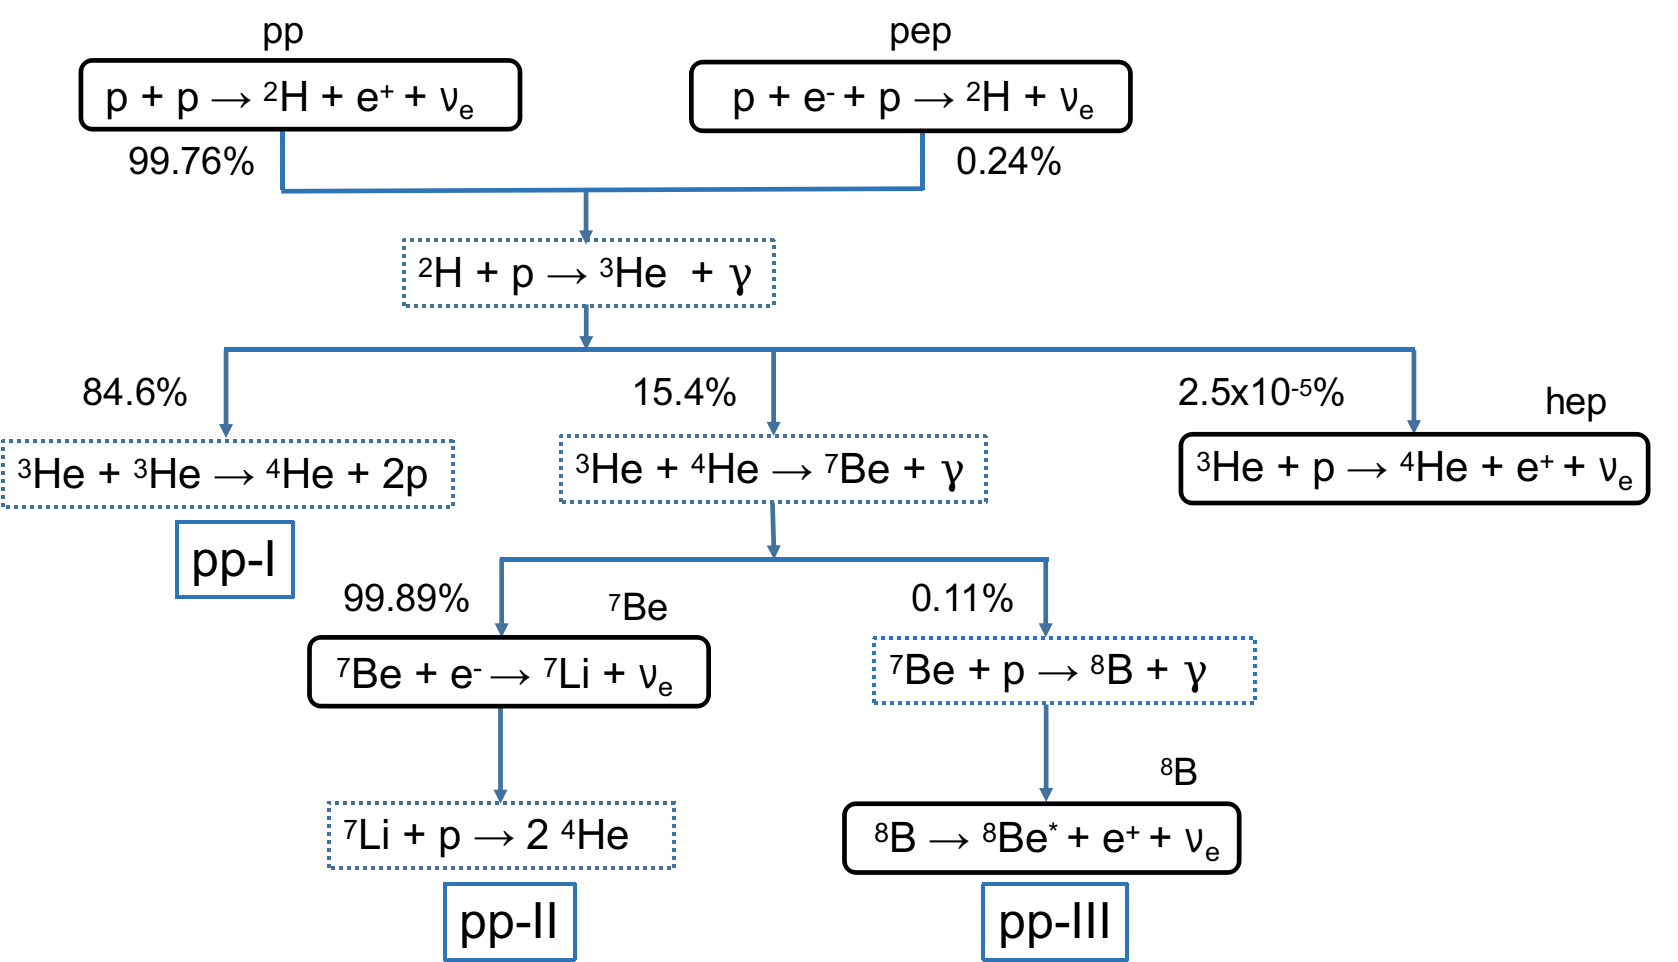
\includegraphics[width=14cm]{ppChain.png}
	\caption[All reactions in the three PP chains.]{All reactions in the three PP chains: PP-I, PP-II, PP-III. The reactions producing neutrinos are labeled in the solid frames. Modified from \cite{oberauer2020solar}.	\label{fig:ppChain}}
\end{figure}

\begin{figure}[htbp]
	\centering	
	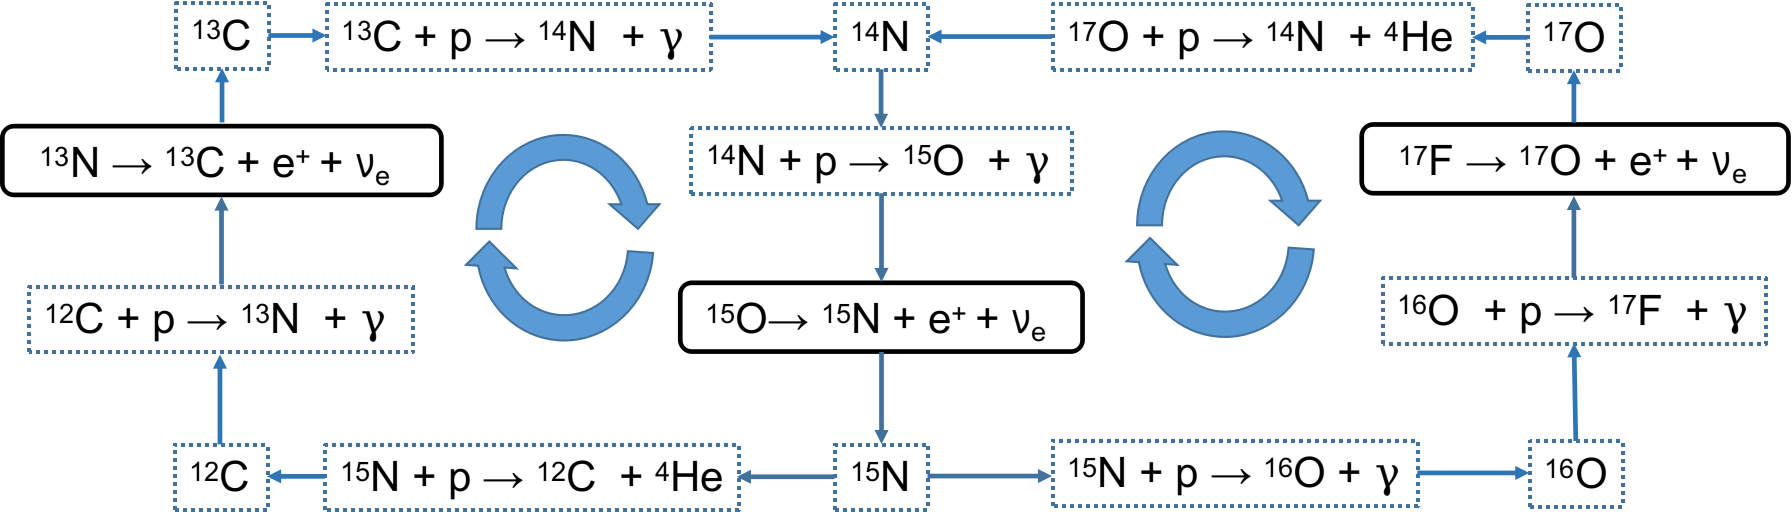
\includegraphics[width=14cm]{CNOcycle.png}
	\caption[All reactions in the CNO bicycle.]{All reactions in the CNO bicycle. The reactions producing neutrinos are labeled in the solid frames. Modified from \cite{oberauer2020solar}.	\label{fig:CNOcycle}}
\end{figure}

Via these nuclear reactions, hydrogen is eventually fused into helium, and the net nuclear transformation is $4p+2e^-\to^{4}$He $+2\nu_e+Q$, where the released energy $Q=26.73$ MeV is mostly in the form of the kinetic energy of the photons, with a small fraction carried by neutrinos\cite{antonio2018state,valle2015neutrinos}.

The electron neutrinos $\nu_e$ produced in the solar nuclear reactions are called ``solar neutrinos'' and they can be detected on the Earth. Due to the branching ratios and unterminated chains in the pp chain and CNO cycle, the solar neutrinos come from different reactions, as shown in Fig.~\ref{fig:ppChain} and Fig.~\ref{fig:CNOcycle}. They are named after the corresponding reactions, as shown in Table.~\ref{tab:solarNu}.

\begin{table}[htp]
	\caption[The main reactions produce solar neutrinos.]{The main reactions produce solar neutrinos in pp chain (a) and CNO cycle (b).\label{tab:solarNu} }	
	\subfigure[pp chain]{
		\begin{tabular*}{65mm}{cc}
			\toprule 
			solar $\nu_e$  & reaction  \\
			\midrule
			pp & $p+p\to ^2$H $+e^++\nu_e$ \\
			pep & $p+e^-+p\to^2$H $+~\nu_e$ \\
			hep &  $^3$He $+~p\to^4$He $+~e^++\nu_e$ \\ 
			$^7$Be &  $^7$Be $+~e^-\to^7$Li $+~\nu_e$\\
			$^8$B & $^8$B$\to^8$Be$^*+e^++\nu_e$\\
			\bottomrule	
		\end{tabular*}
	}
	\subfigure[CNO cycle]{
		\begin{tabular*}{65mm}{cc}
			\toprule 
			solar $\nu_e$   & reaction \\
			\midrule
			CNO &$^{13}$N$\to^{13}$C$+e^++\nu_e$\\	
			& $^{15}$O$\to^{15}$N$+e^++\nu_e$ \\
			& $^{17}$F$\to^{17}$O$+e^++\nu_e$ \\
			\bottomrule	
		\end{tabular*}
	}
\end{table}

The average energy of solar $\nu_e$ is calculated by summing over the $E_{\nu_e}$ from the $i^{th}$ reaction chain with a flux of $\Phi_{\nu_e}^i$ and divided by $\Phi^{tot}_{\nu_e}$\cite{antonio2018state}:
\begin{equation}\label{eq:solarNuEaverage}
\langle E_{\nu_e}\rangle = \sum_i E_i \frac{\Phi^i_{\nu_e}}{\Phi^{tot}_{\nu_e}}\approx 0.265~\mathrm{MeV}.
\end{equation}

For every released energy, there are about two $\nu_e$ generated. Then the solar $\nu_e$ flux at the Earth surface can be estimated via the measured solar radiation energy on the Earth surface:
\begin{equation}
\Phi_{\nu_e} \simeq \frac{\mathcal{L}_{\odot}}{4\pi D_\odot^2}\frac{2}{Q-2\langle E_{\nu_e} \rangle}\simeq 6.40\times 10^{10}~\nu_e/cm^2/s,
\end{equation}
where the solar constants $G_{sc}=\mathcal{L}_\odot/(4\pi D^2_\odot)\simeq 0.136$ W/cm$^2$ \cite{suekane2015neutrino}. 

The SSM can predict the fluxes and energies of the solar neutrinos coming from different reactions, as shown in Fig.~\ref{fig:haxton2013plot}\cite{haxton2013solar}.

\begin{figure}[htbp]
	\centering	
	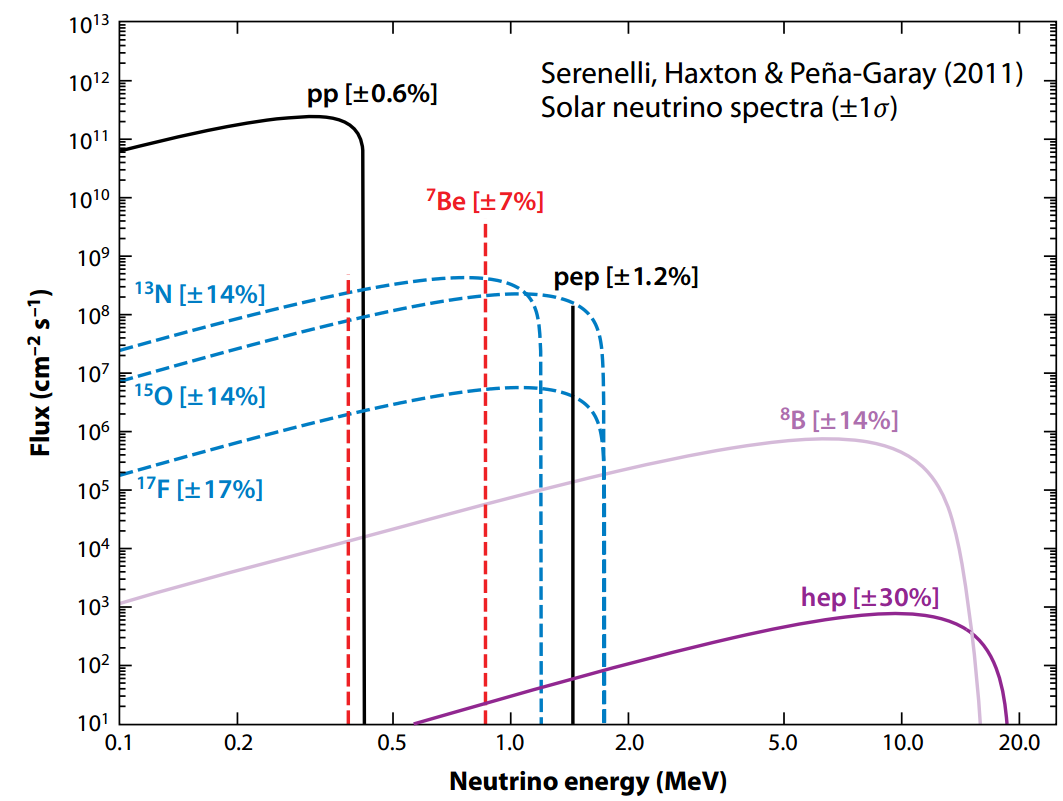
\includegraphics[width=12cm]{haxton09.png}
	\caption[Solar neutrino energy spectrum.]{Solar neutrino energy spectrum ($E_\nu$ vs. flux) along with the SSM uncertainties, from Ref.~\cite{haxton2013solar}.}
	\label{fig:haxton2013plot}
\end{figure}

In 1964, John Bahcall and Raymond Davis proposed the first experiment to detect solar neutrinos\cite{bahcall1964solar,davis1964solar}. Raymond Davis designed an experiment that used a 380 m$^3$ tank filled with Perchloroethylene (C$_2$Cl$_4$), a dry-cleaning fluid rich in chlorine. Solar neutrinos were expected to change $^{37}$C1 to $^{37}$Ar via the endothermic reaction: $\nu_e+^{37}$Cl$\to^{37}$Ar$+e^-$, and the produced $^{37}$Ar were extracted and counted, which is called the radiochemical method. The neutrino energy threshold ($E_{thresh}$) of the experiment was 0.814 MeV, which allowed a measurement mostly of the $^8$B solar $\nu_e$ flux but also including some lower energy neutrinos\cite{davis1964solar}. Their first results, announced in 1968, showed that only about one-third of the predicted radioactive argon atoms were measured\cite{davis1968search}. This pioneering experiment raised a problem of missing solar neutrinos, which is denoted as the solar neutrino problem.

\subsection{Kamiokande and Super-Kamiokande}\label{sect:superKsolarnu}
The solar neutrino problem was later confirmed by the Kamiokande-II experiment in 1988\cite{superKwebsite}. As the successor of the Kamiokande, Super-K uses a 50-kilotonne water Cherenkov detector to measure the solar neutrinos via the $\nu-e^-$ elastic scattering. By utilizing the patterns of the Cherenkov lights produced by the recoil electrons (see Sect.~\ref{sect:cherenkov}, Chapter 3), the direction of the incoming neutrino can be traced and thus the neutrinos from the Sun can be selected. Unlike the radiochemical method, this enables real-time measurements of the solar neutrinos.

In 2000, Super-K reported the observed solar neutrino flux was about 45\% of the expected flux in SSM with more than 99.9\% confidence level, suggesting the flavor transformation of solar neutrinos and limiting the oscillation parameters ($\Delta m^2_{21}$, $\theta_{12}$)\cite{superKwebsite}. 

Super-K continues to measure solar neutrinos with more precision and high statistical accuracy and it is able to lower down the energy threshold to 3.5 MeV to search for the $^8$B solar neutrinos. The fourth phase of Super-K (Super-K-IV) took data from 2008 to 2014, and by utilizing this 1664 live-day data, Super-K-IV reported a measurement of the elastic scattering flux as: $\Phi_{ES}=(2.308\pm0.020(stat.)^{+0.039}_{-0.040}(syst.))\times 10^6~\mathrm{cm^{-2}s^{-1}}$\cite{abe2016solar}. Combined with the previous three phases, it gives $\Phi_{ES}=(2.345\pm0.014(stat.)\pm 0.036(syst.))\times 10^6~\mathrm{cm^{-2}s^{-1}}$\cite{abe2016solar}. These values will be compared to the measurement of this thesis in Sect.~\ref{sect:solarESresults}, Chapter 6.

\subsection{SNO}
It was the Sudbury Neutrino Observatory (SNO) experiment finally resolved the solar neutrino problem and first confirmed that the missing solar neutrinos are due to the neutrino flavor transformation $\nu_e\to\nu_{\mu,\tau}$, along with the matter effect mentioned in Sect.~\ref{sect:MSW}. 

SNO used a 1-kilotonne heavy water (D$_2$O) Cherenkov detector to distinguish the flavors of solar neutrinos. The SNO detector was sensitive to the $^8$B solar neutrinos via three interactions: (1) the charged current (CC) on deuteron ($d$):
$\nu_e+d\to p+p+e^-$, (2) the neutral current (NC): $\nu_x+d\to p+n+\nu_x$, and (3) the elastic scattering (ES): $\nu_x+e^-\to \nu_x+e^-$. The CC channel was only sensitive to $\nu_e$ while the NC channel was independent of the neutrino type (``flavor-blind''), which provided a measurement of the total solar neutrino flux regardless of neutrino flavors. The ES channel was also sensitive to all flavors but with reduced sensitivities to $\nu_\mu$ and $\nu_\tau$\cite{ahmad2002direct}. As mentioned in Sect.~\ref{sect:nuInteraction}, the ES cross-section of $\nu_e$ is 6.5 times larger than the $\nu_{\mu,\tau}$. 

In 2002, SNO reported that the measured total $^8$B solar neutrino flux
via the NC channel ($\Phi_{NC}$) was consistent with the SSM while the $\nu_e$
component of the flux ($\Phi_e$) was about one-third of the total flux\cite{ahmad2002direct}:
\begin{equation}
R = \Phi_{CC}/\Phi_{NC} = \Phi_e/\Phi_{tot}=0.34\pm 0.04.
\end{equation}

A combined analysis of SNO data acquired from 1999 to 2006 gave the measured total flux of $^8$B solar neutrinos by $\Phi_{^8\mathrm{B}}=5.25\pm0.16(stat.)^{+0.11}_{-0.13}(syst.)$ cm$^{-2}$s$^{-1}$. Based on a two-flavor neutrino oscillation analysis, $\Delta m^2_{21}=(5.6^{+1.9}_{-1.4})\times 10^{-5}$ eV$^2$ and $\tan^2\theta_{12}=0.427^{+0.033}_{-0.029}$.
\cite{aharmim2013combined}.

\subsection{Combined Analysis of Solar and Reactor Measurements}
As mentioned in Sect.~\ref{sect:VacuumOsci}, the reactor antineutrino experiments study the neutrino flavor transformation by measuring $\mathcal{O}$(MeV) $\bar{\nu}_e$ produced from reactors. If the distance between the reactor and the detector is long enough (according to Eqn.~\ref{oscillationCondition}, $L\sim\mathcal{O}(100$~km)), such experiments can probe the $\Delta m^2_{12}$ and $\theta_{12}$ parameters, or the flavor transformation parameters in the solar sector. KamLAND is able to study the solar sector due to its long baseline of 180 kilometers (the average value of the distances to the various reactors). It is a 1-kilotonne liquid scintillator detector, located in Gifu Prefecture, Japan, under Mount Ikenoyama at a depth of about 2700 $m.w.e$\cite{abe2008precision}.

Assuming the CPT invariance, the KamLAND and solar neutrino data can be combined by including solar $\nu_e$ and reactor $\bar{\nu}_e$ data to obtain the oscillation parameters.
$\Delta m^2_{21}$

A global analysis including solar and reactor data gives ($1-\sigma$ limits)\cite{oberauer2020solar}:
$0.291<\sin^2\theta_{12}<0.318$,
$7.20\times 10^{-5}\mathrm{eV}^2<\Delta m^2_{12}<7.51\times 10^{-5}\mathrm{eV}^2$.

\subsection{Borexino}
Borexino is a liquid scintillator neutrino detector with a target mass about 300 tonne. It is located at the Gran Sasso National Laboratory (LNGS) in central Italy, under an overburden of rock with 3800 water equivalent meter (m.w.e) to suppress the cosmogenic backgrounds. It is the first experiment that made real-time measurements of the low energy ($<1$ MeV) solar neutrinos, thanks to the high light yield of the liquid scintillator.

Unlike the water Cherenkov detector, though liquid scintillator can provide more photons per deposit energies, it cannot be used to measure the event direction (see Sect.~\ref{sect:scintillator}, Chapter 3). Borexino mainly measures the energy spectrum of the recoil electrons from the $\nu+e^-$ ES, which is called spectroscopic measurement\cite{agostini2020improved}.


Borexino has measured $^7$Be, pep, pp and $^8$B solar neutrino fluxes\cite{agostini2018comprehensive}. 

In 2020, Borexino reported the first observation of CNO neutrino\cite{borexino2020experimental}. interaction rate is $7.2^{+3.0}_{-1.7}$ counts per day per 100 tonnes of target at 68\% C.L. This result gives a flux on Earth of $7.0^{+3.0}_{-2.0}\times 10^8$ cm$^{-2}$s$^{-1}$.

%
%Borexino problems:
%(1)$^{11}$C nuclei induced by the high energy cosmic muon spallation reactions cause a large background contribution. While for SNO+, since it is located at SNOLAB and more deeper,  \cite{whitepaper}.
%(2)intrinsic $\beta$-decays from $^{210}$Bi contaminate the fiducial volume 

\subsection{More Studies on Solar Neutrino and Future Experiments}
%%% Since neutrinos' extremely low interaction cross-sections, neutrinos produced in the Sun can reach the detectors on the Earth without being interrupted. Since neutrinos' extremely low interaction cross-sections, neutrinos produced in the Sun can reach the detectors on the Earth without being interrupted. 
There are three aspects for the solar neutrino research in the future: (1) precision measurements of solar neutrino fluxes, (2) 
sub-leading effects on the phenomenology from both standard and nonstandard physics, and (3) new detection techniques\cite{antonio2018state}.

Precise measurements of low energy solar neutrinos can probe the details of the matter effects, 

Tensions between the reactor and solar experiments
	
Solar metallicity problem.
	
	The SSM predictions are agreed with the helioseismological measurements\cite{gann2015everything,oberauer2020solar}. 
	
	the speed of sound with helioseismological measurements. 
	
Day/night effect
	
	For a solar neutrino detector in the nighttime, solar neutrinos are expected to pass through the Earth's matter before reaching the detector, while in the daytime 
	
	
	
	   
	 they are expected 
	
	 
	
	This effect has been measured by several experiments, such as SNO\cite{aharmim2013combined} and Super-K\cite{abe2016solar}.
	
	which was
statistically limited and not definitive\cite{abe2016solar,suzuki2020sun}.
	
Non-standard neutrino interaction (NSI)   
	
Dark matter in the Sun


There are a few new experiments being planned to precisely measure the solar neutrinos in the near future. These experiments include large water Cherenkov detector like Hyper-Kamiokande (Hyper-K), large liquid scintillator detectors like JUNO, Jinping and ASDC-THEIA, and ton-scale dark matter direct search detectors. 

New techniques of liquid scintillator, 

Hyper-Kamiokande (Hyper-K) is the successor of Kamiokande and Super-K. As a water Cherenkov detector with a fiducial mass of 187 kilotonne, which is about 8 times larger than the Super-K and expects to observe 130 $\nu+e^-$ elastic scattering events per day. It is aimed for a detection of $hep$ solar neutrino flux, which has not been detected yet. Also, the expected large statistics ob

 can resolve the $2-\sigma$ discrepancy of neutrino mass squared difference between the solar and reactor experiments. 

ASDC-THEIA and Jinping Neutrino Experiment (Jinping)\cite{beacom2017physics}

water-based liquid scintillator 
doping

Sect.~\ref{sect:wbWLS}.

is planned to build a 4-kilotonne liquid scintillator or water-based liquid scintillator detector at China Jinping Underground Laboratory (CJPL), 
Its fiducial mass for the $\nu-e^-$ scattering events is proposed to be 2 kiloton, which is 20 times larger than the Borexino target mass. With the advantages of low cosmogenic backgrounds and large fiducial mass target, Jinping is featured to measure pp neutrinos in the range of 0.2-0.3 MeV, $^7$Be, pep and CNO neutrinos
can for a 5-year run\cite{beacom2017physics}. 

With the improving sensitivities, ton-scale dark matter direct search experiments, such as the DARWIN experiment (DARk matter WImp search with liquid xenoN), will be able to detect neutrino interactions\cite{aalbers2016darwin}. With energy threshold down to several keV and ultra-low background level, DARWIN will have the potential to measure low-energy solar neutrinos via $\nu-e^-$ elastic scattering, especially for the pp and $^7$Be solar neutrinos. 1 keV with 1\% precision\cite{baudis2014neutrino,aalbers2020solar}.

DUNE

Among these experiments, SNO+ has measured $^8$B solar neutrino flux in its initial water phase. In the next scintillator phase, SNO+ is able to measure low energy solar neutrinos ($E_\nu<2$ MeV), especially for the CNO and $pep$ neutrinos. Due to the depth of SNOLAB (will be discussed in Sect.~\ref{sect:overview}, Chapter 3), SNO+ is expected to have much lower cosmogenic backgrounds than the Borexino, and thus may obtain more precise measurements\cite{directorReview}. 

\section{Neutrinoless Double Beta Decay}\label{sect:doublebeta}
The neutrino flavor transformation experiments proved that neutrinos are not massless and have finite masses. However, in these experiments, the mass differences, rather than the absolute mass values are measured so we can not know the absolute scale of neutrino masses from these results. Currently, there are mainly three approaches to probe the neutrino masses\cite{valle2015neutrinos}: (1) Cosmological measurements\cite{aghanim2020planck,dvorkin2019neutrino,lesgourgues2013neutrino}; (2) Direct measurements of the $\beta$-decay spectrum; and (3) A search for the neutrinoless double beta decay ($0\nu\beta\beta$) process, which will be discussed below.

For heavy radioactive isotopes ($A>70$) with nuclei of even neutron number and even proton number (called the even-even nucleus), beta decay will lead to an odd-odd nucleus which is less stable. Thus for such isotopes, the $\beta$-decay is energetically forbidden. In 1935, Maria Goeppert-Mayer pointed out that these isotopes can still decay through a double beta decay process: $(Z,A) \to (Z+2,A)+2e^{-}+2\bar{\nu}_e+Q_{\beta\beta}$, where $Q_{\beta\beta}$ is the released energy. This is called ordinary double beta decay or $2\nu\beta\beta$, which is allowed by the SM and with a typical half-life $T_{1/2}>10^{19}$ years (yr)\cite{povh2008particles,martin2019nuclear}.

In the SM, neutrinos are fermions without carrying electrical charges. A conjecture raised up is that they could be ``truly neutral'', i.e., no charge-like quantum number can be used to distinguish a neutrino and an antineutrino\cite{akhmedov2014majorana}. Such a neutral fermion 
that is its own antiparticle, is called Majorana particle, which was proposed by Ettore Majorana based on a mathematical modification of the Dirac equation\cite{majorana2006symmetric}.

Proposed by W.H.Furry in 1939\cite{furry1939transition}, if neutrinos are Majorana particles (Majorana neutrinos), a process called neutrinoless double beta decay ($0\nu\beta\beta$) will also be expected: $(Z,A) \to (Z+2,A)+2e^{-}+Q_{\beta\beta}$. In this process, the lepton number is violated by 2, which is not allowed in the SM and New Physics interpretations are required. The Feynman diagrams of $2\nu\beta\beta$ and $0\nu\beta\beta$ are illustrated in Fig.~\ref{feynman1}.
\begin{figure}[htbp]
	\centering
	{	
		\begin{minipage}[t]{0.45\textwidth}{(a)}
			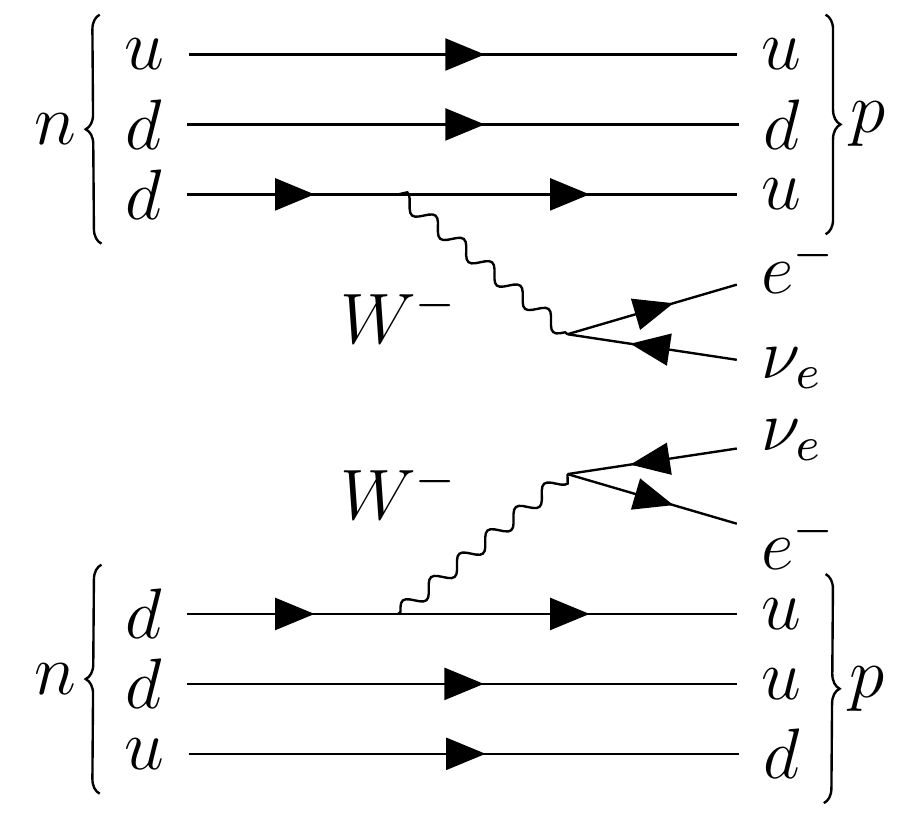
\includegraphics[width=5cm]{doubleBeta2nu_feynman.png}
		\end{minipage}
		\begin{minipage}[t]{0.45\textwidth}{(b)}
			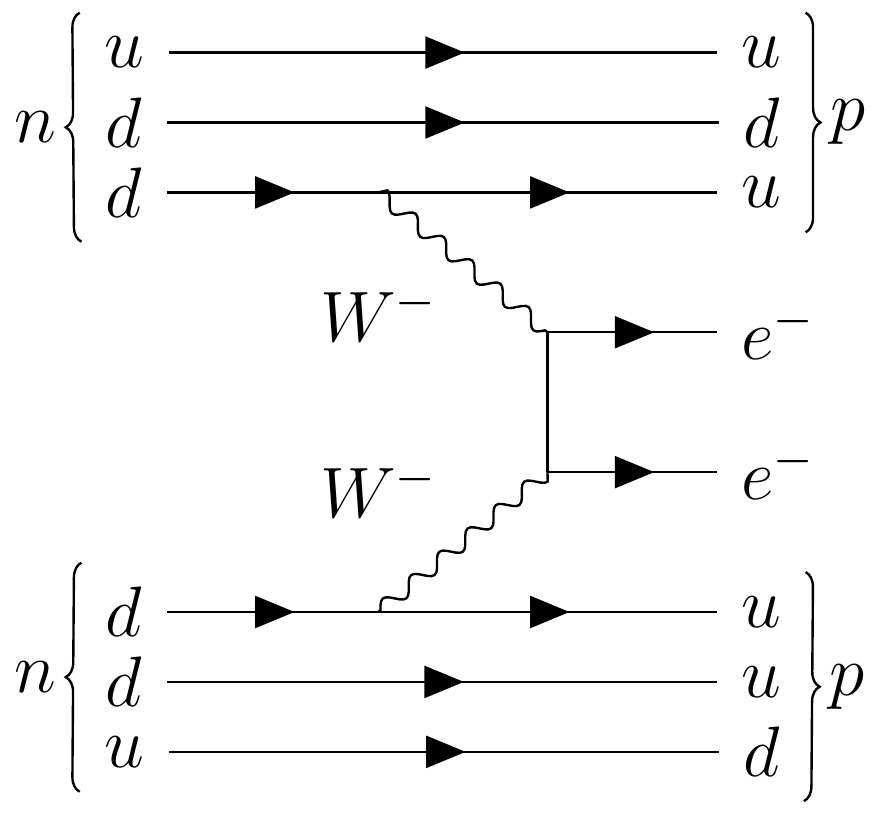
\includegraphics[width=5cm]{doubleBeta_feynman.png}
		\end{minipage}
		\caption[Feynman diagrams for $2\nu\beta\beta$ and $0\nu\beta\beta$.]{Feynman diagrams for $2\nu\beta\beta$ (a) and $0\nu\beta\beta$ (b).}
		\label{feynman1}
	}
\end{figure}

For the Majorana neutrino, an effective Majorana mass $\langle m_{ee}\rangle$ is defined as\cite{suekane2015neutrino,zuber2020neutrino}:
\begin{equation}\label{eq:effective_nuMass}
\langle m_{ee}\rangle = |\sum_{i=1}^3 U^2_{ei}m_i|= |c^2_{13}c^2_{12}m_1+c^2_{13}s^2_{12}e^{i\alpha_1}m_2+s^2_{13}e^{i\alpha_2}m_3|,
\end{equation}
where the values of $U_{ei}$ are the elements of the neutrino mixing matrix for the flavor state $\nu_e$, and $m_i$ are the mass eigenvalues of the mass eigenstates, according to Enq.~\ref{eq:mixingmatrix}; $\alpha_1,\alpha_2$ are two Majorana CP-violation phase factors ranging from 0 to $\pi$, and $\alpha_2$ can also be taken as $\alpha_2-\delta_{CP}$.

The neutrino mass eigenvalues $m_i$ can be expressed as the lightest neutrino mass $m_{lightest}$ and mass square differences $\Delta m^2_{ij}$\cite{suekane2015neutrino}:

for the NH, $m_{lightest}=m_1$, and $m_2=\sqrt{m_{lightest}^2+\Delta m^2_{21}}, m_3 = \sqrt{m_{lightest}^2+|\Delta m^2_{31}|}$;

for the IH, $m_{lightest}=m_3$, $m_1=\sqrt{m_{lightest}^2+|\Delta m^2_{31}|}, m_2=\sqrt{m_{lightest}^2+|\Delta m^2_{31}|+\Delta m^2_{21}}$.

In this case, the effective Majorana mass can be expressed as the $m_{lightest}$ and neutrino flavor transformation parameters $\theta_{ij}$ and $\Delta m^2_{ij}$. A probe of the $\langle m_{ee}\rangle$ can thus determine the $m_{lightest}$ and then determine the absolute neutrino masses. 

The decay width and the half-life of the $0\nu\beta\beta$ process are calculated as\cite{suekane2015neutrino,zuber2020neutrino}:
\begin{equation}\label{eq:decayWidth0vbb}
\Gamma=(T^{0\nu}_{1/2})^{-1} = G_{PS}(Q,Z)|M_{Nuclear}|^2\langle m_{ee}\rangle^2, 
\end{equation}
where $G_{PS}(Q,Z)$ is a phase space corresponding to the effective coupling constant, which depends on the endpoint energy $Q$ and the atomic number $Z$; $|M_{Nuclear}|$ is the nuclear matrix element describing the nuclear transition and it can only be calculated theoretically from approximate methods based on many-body nuclear models, such as the Nuclear Shell Model (NSM), interacting Boson Model (IBM), etc. Since the $G_{PS}$ and $|M_{Nuclear}|^2$ can be calculated theoretically, an $0\nu\beta\beta$ experiment measures the $T^{0\nu}$ to quantify the $\langle m_{ee}\rangle$.

Similar to the $\beta$-decay case, the $2\nu\beta\beta$ process will cause a continuous spectrum in the detector while the $0\nu\beta\beta$ process only has two electrons in the final state. These electrons take away the total energy (the energy from the nuclear recoil is negligible here), and their energy spectra sum up to give a distinct energy peak at the Q-value ($Q_{\beta\beta}$). Taking the isotope $^{130}$Te as an example, Fig.~\ref{te130energy} illustrates the shapes of the energy spectrum from the $2\nu\beta\beta$ and the $0\nu\beta\beta$ decay processes.
\begin{figure}[htbp]
	\centering	
	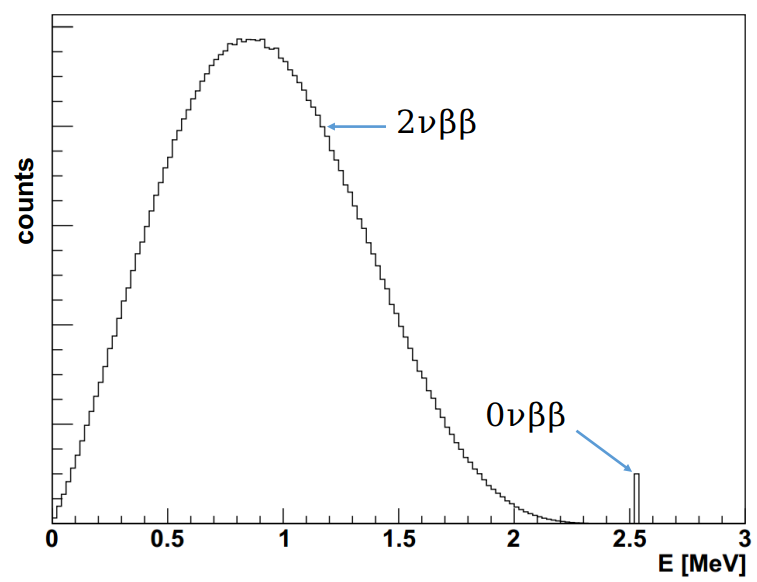
\includegraphics[width=8cm]{Te130_energy0vbb.png}
	\caption[Energy spectrum of the $^{130}$Te $2\nu\beta\beta$ decay and the hypothetical $0\nu\beta\beta$ decay.]{Energy spectrum of the $^{130}$Te $2\nu\beta\beta$ decay and the hypothetical $0\nu\beta\beta$ decay. The SNO+ software package (\texttt{RAT}) was used to produce the simulations for the plot. The package is described in Sect.~\ref{sect:rat}.}
	\label{te130energy}
\end{figure}

To determine the $T^{0\nu}_{1/2}$, experiments search for events appearing around the $Q_{\beta\beta}$. For a candidate isotope, the observed number of events in expectation is: 
\begin{equation}
N_{event} = \ln 2 \frac{N_A}{M_A}\frac{\alpha\cdot\epsilon\cdot m\cdot t}{T^{0\nu}_{1/2}},
\end{equation}
where $N_A$ is the Avogadro's number, $\alpha$ is the abundance of the isotope in the element, $M_A$ is the molar mass of the isotope, $m$ is the target isotope mass in the detector, and $t$ is the measurement time of total exposure.

There are 35 candidate isotopes can undergo the $2\nu\beta\beta$ decay process, but only a few of them are suitable for the application in direct $0\nu\beta\beta$ search experiments\cite{giunti2007fundamentals}. From the experimental view, the candidate isotopes are expected to have relatively high natural abundances and high Q-values, be deployed in a large amount with low costs, be atoxic and unharmful to the environment, etc. However, in a realistic situation, no isotope fulfills all these criteria, and trade-offs have to be made for the current experiments\cite{dolinski2019neutrinoless}. Fig.~\ref{fig:te_abundance} shows the Q-values and natural abundances of the candidate isotopes currently selected by the $0\nu\beta\beta$ experiments.

\begin{figure}[!htb]
	\centering
	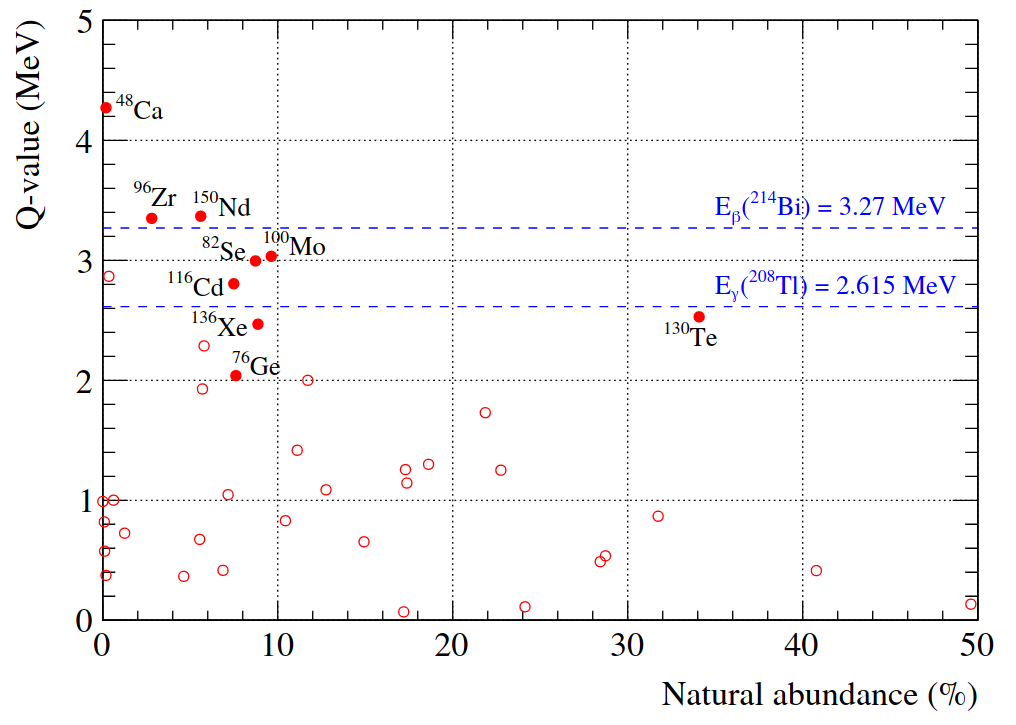
\includegraphics[width=10cm]{Te_abundance.png}
	\caption{Natural abundance vs. Q-values for different $2\nu\beta\beta$ isotopes, from Ref.~\cite{snop_nim_draft}.}
	\label{fig:te_abundance}
\end{figure}

Among these isotopes, $^{130}$Te has the highest natural abundance of 34\% and thus can provide a higher target isotope mass. SNO+ will use Te-loaded liquid scintillator to search for $0\nu\beta\beta$, which will be discussed in Chapter 3. 

At the time of this writing, no experiment has found the signal of $0\nu\beta\beta$, while limits on $T^{0\nu}_{1/2}$ and $\langle m_{ee}\rangle$ for various candidate isotopes have been setting. Currently, the best limit of $T^{0\nu}_{1/2}$ reported by the experiments is obtained from the KamLAND-Zen (ZEroNeutrino) Experiment, searching for the signal from the $^{136}$Xe. Their 2016 results gave a lower limit of $T^{0\nu}_{1/2}(^{136}$Xe$)>1.07\times 10^{26}$ yr at 90\% C.L., and the corresponding upper limits on the effective Majorana mass: $\langle m_{ee}\rangle<(61-165)$ meV\cite{gando2016search}. 

For $^{130}$Te, the current best limit is from the CUORE experiment (Cryogenic Underground Observatory for Rare Events). In 2018, CUORE placed a lower limit of $T^{0\nu}_{1/2}(^{130}$Te$)>1.5\times 10^{25}$ yr at 90\% C.L., and $\langle m_{ee}\rangle<(110-520)$ meV\cite{alduino2018first}.

For $^{76}$Ge, the current best limit is from the GERDA experiment (GERmanium Detector Array). In 2019, GERDA reported a lower limit half-life of $T^{0\nu}_{1/2}(^{76}$Ge$)>1.8\times 10^{26}$ years at 90\% C.L. with $\langle m_{ee}\rangle<(79-180)$ meV\cite{agostini2020final}.

Future experiments in a decade, such as the KamLAND2-Zen, LEGEND-1000, nEXO, are expected to reach $T^{0\nu}_{1/2}$ at $\mathcal{O}(10^{27}-10^{28})$ years\cite{dolinski2019neutrinoless}.